\documentclass[a4paper,twoside,11pt]{article}
\usepackage{a4wide,algo,graphicx,fancyhdr,amsmath,amssymb,amsthm,ifthen,path,todonotes}
\usepackage{subcaption, caption}
\usepackage[ruled, noline, algo2e, noend]{algorithm2e}
\usepackage{hyperref}
\usepackage{url}
\usepackage{color}
\urlstyle{rm}
\usepackage{tikz}
\usepackage{xifthen}
\usepackage{listings}
\usepackage{pgfplots}
\usepackage{comment}
\usepackage{parskip}
\usepackage{tabularx, colortbl}
\usepackage{mathtools}
\usepackage{amsmath}
\usepackage{float}
%----------------------- Macros and Definitions --------------------------
\graphicspath{ {./img/} }

\setlength\headheight{10pt}
\addtolength\topmargin{-10pt}
\addtolength\footskip{20pt}

\newenvironment{myindentpar}[1]%
{\begin{list}{}%
	{\setlength{\leftmargin}{#1}}%
	\item[]%
}
 {\end{list}}

\fancypagestyle{plain}{
\fancyhf{}
\fancyfoot[LO,RE]{\sffamily\bfseries Eindhoven University of Technology}
\fancyfoot[RO,LE]{\sffamily\bfseries\thepage}
\renewcommand{\headrulewidth}{0pt}
\renewcommand{\footrulewidth}{0pt}
}

\newcommand{\List}{\mathcal{L}}
\newcommand{\T}{\mathcal{T}}
\newcommand{\G}{\mathcal{G}}
\newcommand{\s}{\mathcal{S}}

\newcommand{\opt}{\textsc{opt}}

\pagestyle{fancy}
\fancyhf{}
\fancyhead[LE]{\sffamily\bfseries }
\fancyhead[RO]{\sffamily\bfseries Project1 - Particles}
\fancyfoot[LO,RE]{\sffamily\bfseries 2IV15 Simulation in computer graphics - Eindhoven University of Technology}
\fancyfoot[RO,LE]{\sffamily\bfseries\thepage}

%-------------------------------- Title ----------------------------------

\title{\sffamily\bfseries
Project1 \\[1ex]
\large Fluids
}

\author{
    Wouter Lok \\
    Student number: 0832518 \\
    \texttt{w.lok@student.tue.nl}
    \and
    Joris Reijrink \\
    Student number: 0847198 \\
    \texttt{j.reijrink@student.tue.nl}\\
}

\date{\today}

\setlength{\parindent}{24pt}

% Set \item separation length
%\newlength{\wideitemsep}
%\setlength{\wideitemsep}{1\itemsep}
%\addtolength{\wideitemsep}{-7pt}
%\let\olditem\item
%\renewcommand{\item}{\setlength{\itemsep}{\wideitemsep}\olditem}


%--------------------------------- Text ----------------------------------

\begin{document}

\maketitle
\newpage

\vspace{1cm}

\section{Introduction}
In this report, we describe the results of the implementation of a particle system with constraints. The system is able to solve and simulate forced applied to particles while taking into account the constrains of the particles. Forces and constraints are applied in a generalized structure such that new forces and constraints can be added easily.
\section{Results}
In the figures below some scenes are shown of the final result.

\begin{figure}[h!]
\centering
\begin{minipage}[t]{.40\textwidth}
  \centering
  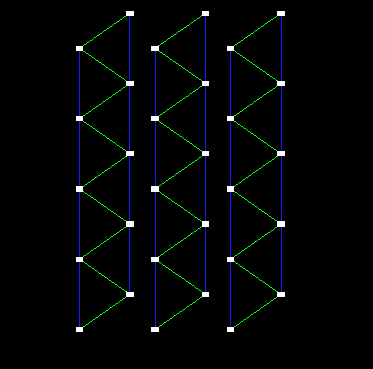
\includegraphics[height=5cm]{img/resulthair.png}
  \captionof{figure}{Start position of hair}
  \label{fig:hair}
\end{minipage}\hfill
\begin{minipage}[t]{.50\textwidth}
  \centering
  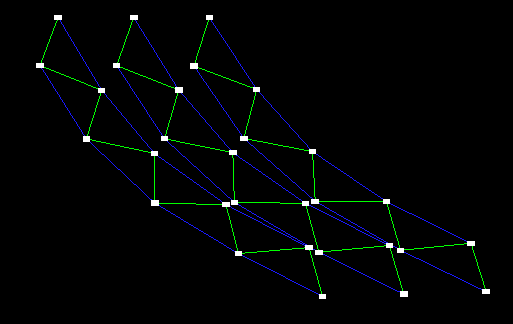
\includegraphics[height=5cm]{img/resulthair2.png}
  \captionof{figure}{Hair position after some iterations}
  \label{fig:hair2}
\end{minipage}
\end{figure}

\begin{figure}[h!]
\centering
\begin{minipage}[t]{.45\textwidth}
  \centering
  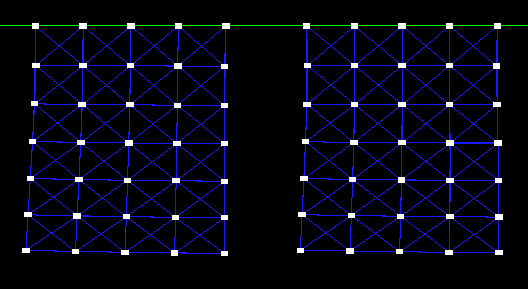
\includegraphics[height=4cm]{img/curtain.png}
  \captionof{figure}{Start position of two cloth curtains }
  \label{fig:flag}
\end{minipage}\hfill
\begin{minipage}[t]{.45\textwidth}
  \centering
  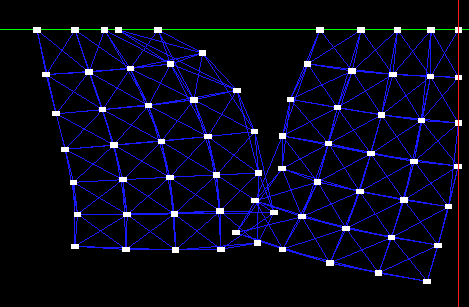
\includegraphics[height=4cm]{img/curtain2.png}
  \captionof{figure}{Two cloth curtains colliding}
  \label{fig:flag2}
\end{minipage}
\end{figure}




\section{Conclusion}

We started with the implementation of a global system to solve all forces and constraints.
With these forces and constraints we made some nice scenes such as hair and cloth, as shown in the results.
The user can also apply forces by interacting with the mouse.
Because the euler integration method is not very stable other integration methods where implemented.
Finally collision detection is implemented such as particle collisions and fixed object collisions.

\end{document}
